%%%%%%%%%%%%%%%%%%%%%%%%%%%%%%%%%%%%%%%%%
% Stylish Article
% LaTeX Template
% Version 2.1 (1/10/15)
%
% This template has been downloaded from:
% http://www.LaTeXTemplates.com
%
% Original author:
% Mathias Legrand (legrand.mathias@gmail.com) 
% With extensive modifications by:
% Vel (vel@latextemplates.com)
%
% License:
% CC BY-NC-SA 3.0 (http://creativecommons.org/licenses/by-nc-sa/3.0/)
%
%%%%%%%%%%%%%%%%%%%%%%%%%%%%%%%%%%%%%%%%%


% +++ Enter the contend in the included files, only configuration in this file +++ 


%----------------------------------------------------------------------------------------
%	PACKAGES AND OTHER DOCUMENT CONFIGURATIONS
%----------------------------------------------------------------------------------------

% #NOTE change back to 10pt if the paper is longer than 5 pages
\documentclass[fleqn,11pt]{SelfArx} % Document font size and equations flushed left

\usepackage[english]{babel} % Specify a different language here - english by default

\usepackage{lipsum} % Required to insert dummy text. To be removed otherwise


% Command for source
\newcommand{\source}[1]{\caption*{Source: {#1}} }
%----------------------------------------------------------------------------------------
%	COLUMNS
%----------------------------------------------------------------------------------------

\setlength{\parindent}{0pt}
\setlength{\columnsep}{0.55cm} % Distance between the two columns of text
\setlength{\fboxrule}{0.75pt} % Width of the border around the abstract

%----------------------------------------------------------------------------------------
%	COLORS
%----------------------------------------------------------------------------------------

\definecolor{color1}{RGB}{0,0,90} % Color of the article title and sections
\definecolor{color2}{RGB}{0,20,20} % Color of the boxes behind the abstract and headings

\usepackage{soul}

%----------------------------------------------------------------------------------------
%	HYPERLINKS
%----------------------------------------------------------------------------------------

\usepackage{hyperref} % Required for hyperlinks
\hypersetup{hidelinks,colorlinks,breaklinks=true,urlcolor=color2,citecolor=color1,linkcolor=color1,bookmarksopen=false,pdftitle={Title},pdfauthor={Author}}

%----------------------------------------------------------------------------------------
%	ARTICLE INFORMATION
%----------------------------------------------------------------------------------------

\JournalInfo{Robotics and Navigation in Medicine 2019} % Journal information
\Archive{} % Additional notes (e.g. copyright, DOI, review/research article)

\PaperTitle{Image Guided Robotic Transcranial Magnetic Stimulation} % Article title

\Authors{Lennart Kück, Sebastian Engelhardt, Max Haufschild, Sandeep Parameshwara, Pavan Vishwanath} % Authors
% \affiliation{\textsuperscript{1}\textit{Department of Biology, University of Examples, London, United Kingdom}} % Author affiliation
% \affiliation{\textsuperscript{2}\textit{Department of Chemistry, University of Examples, London, United Kingdom}} % Author affiliation
% \affiliation{*\textbf{Corresponding author}: john@smith.com} % Corresponding author

\Keywords{} % Keywords - if you don't want any simply remove all the text between the curly brackets
\newcommand{\keywordname}{Keywords} % Defines the keywords heading name

%----------------------------------------------------------------------------------------
%	ABSTRACT
%----------------------------------------------------------------------------------------

\Abstract{% !TEX root = paper.tex
In this paper, we present a motion compensating system that tracks the patients head movement using a depth camera and moves a coil attached to an industrial robot accordingly. A setup like this can be used for Transcranial magnetic stimulation (TMS), where it is important to keep the coil in a fixed position relative to the head for a longer time period. We developed a functioning implementation of such a system, which achieves an average accuracy of 0.66 cm for a head moving at typical speed.

% \lipsum[1]}

%----------------------------------------------------------------------------------------

\begin{document}

\flushbottom % Makes all text pages the same height

\maketitle % Print the title and abstract box

\tableofcontents % Print the contents section

\thispagestyle{empty} % Removes page numbering from the first page

%----------------------------------------------------------------------------------------
%	ARTICLE CONTENTS
%----------------------------------------------------------------------------------------
% !TEX root = paper.tex
\section{Introduction [LK, MH, SE]}

% \addcontentsline{toc}{section}{Introduction} % Adds this section to the table of contents

Transcranial magnetic stimulation (TMS) is a medical procedure which uses magnetic fields to stimulate a specific cortex region. During this procedure, it is critical to keep the coil fixed to the relevant section of the head.
This usually requires the patient to avoid head movements for up to 30 minutes. However, it was found, that the electric field in the target region is reduced by 32.0\% at the end of the treatment \cite{TMS_Schlaefer}.
Using a robot to place the coil and an image guiding system to maneuver the robot to keep it in the correct position can improve the effectiveness and make it more comfortable for the patient.
We implement such a motion compensating system and evaluate its performance in a physical test setup (fig. \ref{headtrackingsetup}).

\begin{figure}[ht]
	\centering
 	\includegraphics[width=\linewidth]{headtracking_image}
 	\caption{Laboratory test setup}
 	\label{headtrackingsetup}
 \end{figure}
The used methods to create the described motion compensation system are explained in section 2. In the third section we present and discuss our results. A conclusion is drawn in the fourth section.

% \lipsum[1-3] % Dummy text

%------------------------------------------------
% !TEX root = paper.tex

\section{Methods}

% \lipsum[1]
There are three essential problems to be solved. First we solve the robot kinematics. We then implement algorithms for depth camera and hand to eye calibration. Lastly, we implement a procedure for tracking the head and then combine these parts into a single working system.

\subsection{Robot Kinematics [MH]}
In this chapter, both the direct and the inverse kinematics are presented.
The direct kinematics is used for calculating the initial offset between endeffector
and head and for performing the hand-eye calibration. The inverse kinematics is used to
move the robot.
\subsubsection{Direct Kinematics}
The Denavit-Hartenberg (DH) parameters of the UR3 robot are depicted in Fig.~\ref{fig1}.
\begin{figure}[htbp]
\centerline{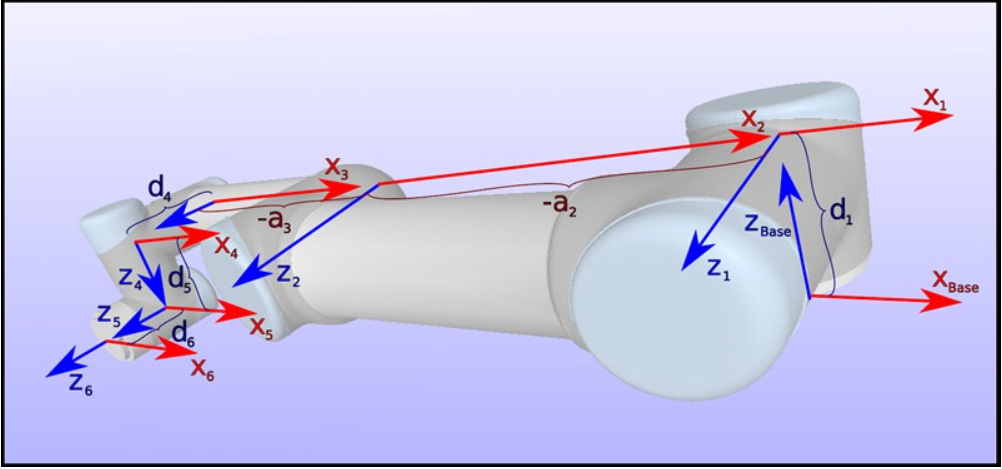
\includegraphics[width=8cm]{DH}}
\caption{DH parameters of the UR3.}
\label{fig1}
\end{figure}

By using the DH convention, the DH parameters can be obtained as shown in table \ref{tab1}.

\begin{table}[htbp]
\caption{DH parameters of the UR3 robot}
\begin{center}
\begin{tabular}{|c|c|c|c|c|}
\hline
\cline{2-5} 
\textbf{joint} & \textbf{\textit{$\theta_{i}$ [deg]}}& \textbf{\textit{$a_{i}$ [m]}}& \textbf{\textit{$d_{i}$ [m]}} & \textbf{\textit{$\alpha_{i}$ [deg]}}\\
\hline
i = 1& $\theta_{1}$& 0& 0.1519& 90 \\
i = 2& $\theta_{2}$& -0.24356& 0& 0 \\
i = 3& $\theta_{3}$& -0.21325& 0& 0 \\
i = 4& $\theta_{4}$& 0& 0.11235& 90 \\
i = 5& $\theta_{5}$& 0& 0.08535& -90 \\
i = 6& $\theta_{6}$& 0& 0.0819& 0 \\
\hline
\end{tabular}
\label{tab1}
\end{center}
\end{table}
The transformation from joint $i$ to joint $i-1$ can be calculated by \eqref{eq1}, where $s_{\alpha_{i}}$ is the short form for $\sin(\alpha_{i})$ and $c_{\alpha_{i}}$ is the short form for $\cos(\alpha_{i})$
\begin{equation}
{}^{i}{T}_{i-1} = \left( \begin{array}{rrrr}                                
c_{\theta_{i}} & -c_{\theta_{i}} \cdot s_{\theta_{i}} & s_{\alpha_{i}} \cdot s_{\theta_{i}} & a_{i} \cdot c_{\theta_{i}} \\                                               
s_{\theta_{i}} & c_{\alpha_{i}} \cdot c_{\theta_{i}} & -s_{\alpha_{i}} \cdot c_{\theta_{i}} &  a_{i} \cdot s_{\theta_{i}} \\                                               
0 & s_{\alpha_{i}} & c_{\alpha_{i}} & d_{i} \\
0 & 0 & 0 & 1 \\                                               
\end{array}\right)
\label{eq1}
\end{equation}

Using \eqref{eq1}, the forward kinematics of the UR3 robot can be calculated 
\begin{equation}
{}^{0}{T}_{6}={}^{0}{T}_{1} \cdot {}^{1}{T}_{2} \cdot {}^{2}{T}_{3} \cdot {}^{3}{T}_{4} \cdot {}^{4}{T}_{5} \cdot {}^{5}{T}_{6}
\label{eq2}
\end{equation}

\subsubsection{Inverse Kinematics}
In general, the inverse kinematics of a 6 degrees of freedom robot can’t be calculated analytically. However, with the geometry of the UR3 robot, there are rotation axes which are parallel to each other or intersecting. As a result, the inverse kinematics gets easier and in the case of the UR3, the inverse kinematics can be solved analytically. The equations and their derivations can be found in $\cite{andersen2018kinematics}$. For the joint angles $\theta_{1}$, $\theta_{3}$ and $\theta_{5}$ one can choose either a positive or a negative sign, which denotes different possibilities to move the robot to the same pose. Because the sign of one angle infuences the value of other angles, there are in general 8 different solutions for the inverse kinematics. This effect can be seen in the equation of $\theta_{5}$ which depends on $\theta_{1}$

\begin{equation}
\theta_{5}=\pm \arccos\left(\frac{{}^{0}{P}_{6x} \cdot \sin(\theta_{1})-{}^{0}{P}_{6y} \cdot \cos(\theta_{1})-d_{4}}{d_{6}}\right)
\label{eq3}
\end{equation}

However, in some constellations fewer than 8 solutions exist because a few solutions are geometrically not possible. The inverse kinematics algorithm makes sure that only the existing solutions are considered and compares them with the current robot position. The existing solution which is closest to the current robot position is then passed to the motion compensation. This solution is found by taking the squared distance of the current joint states and the actual existing solutions.


\subsection{Camera Calibration [SE]}

For the head tracking, a Microsoft Kinect V2 is used. This sensor uses a normal RGB camera combined with an infrared based depth camera. In order to provide accurate tracking, the cameras have to be calibrated. The camera intrinsic calibration is needed to undistort the images. The camera matrix of the RGB camera is also used for the 3D reconstruction in hand-eye calibration. 
As we are using both depth and RGB informations for the tracking, the extrinsic calibration, that means the mapping of the RGB camera to the depth camera, is needed. 
% #TODO do we need source here?

The camera calibration is done using the computer vision library OpenCV \cite{opencv_library}. In order to access the Kinect from ROS, the package IAI Kinect2 \cite{iai_kinect2} is used. The rectification and undistortion process using the calibration parameters is also handled by this software.

\paragraph{Intrinsic Calibration}

The used method for the camera intrinsic calibration is based on the algorithm from Zhang \cite{Zhang}. 
To apply the calibration method, several different image of a know calibration pattern, a chessboard in this case, must be recorded. 
The inputs for that algorithm are then combinations of image points and object points. The image points are the 2D locations of the chessboard corners in each image. The object points represent the calibration pattern and are in 3D in real world space. For simplification, the world coordinate system is assumed to be at the chessboard plane so that the $z$ coordinate is always zero. 

The locations of the image points are first determined by classical image processing 
procedures and then refined in an iterative manner to achieve sub pixel accuracy.
% #TODO more details? We just use an OpenCV function

The depth camera has a much lower resolution than the RGB camera. The images or the calibration of that camera are therefore scaled up using cubic interpolation. Without that the detection of chess bord corners is only possible for small distances.

We use 40 images for the calibration. The OpenCV implementation of the calibration algorithm returns the root mean square (RMS) re-projection error. For the RGB camera we achieved an error of $0.110$ pixels and for the depth camera an error of $0.136$ pixels. 


% \lipsum[1] % Dummy text

\paragraph{Extrinsic Calibration}
As described above, our setup requires a RGB camera to depth camera calibration. During this procedure, the transformation between both cameras is estimated by comparing poses of the calibration pattern relative to the RGB camera and relative to the depth camera. We use the same 80 images as used for the intrinsic calibrations, as they were already taken synchronously. 
 

% \lipsum[1] % Dummy text

\subsection{Hand-Eye Calibration [PV]}
 \begin{figure}[ht]
	\centering
 	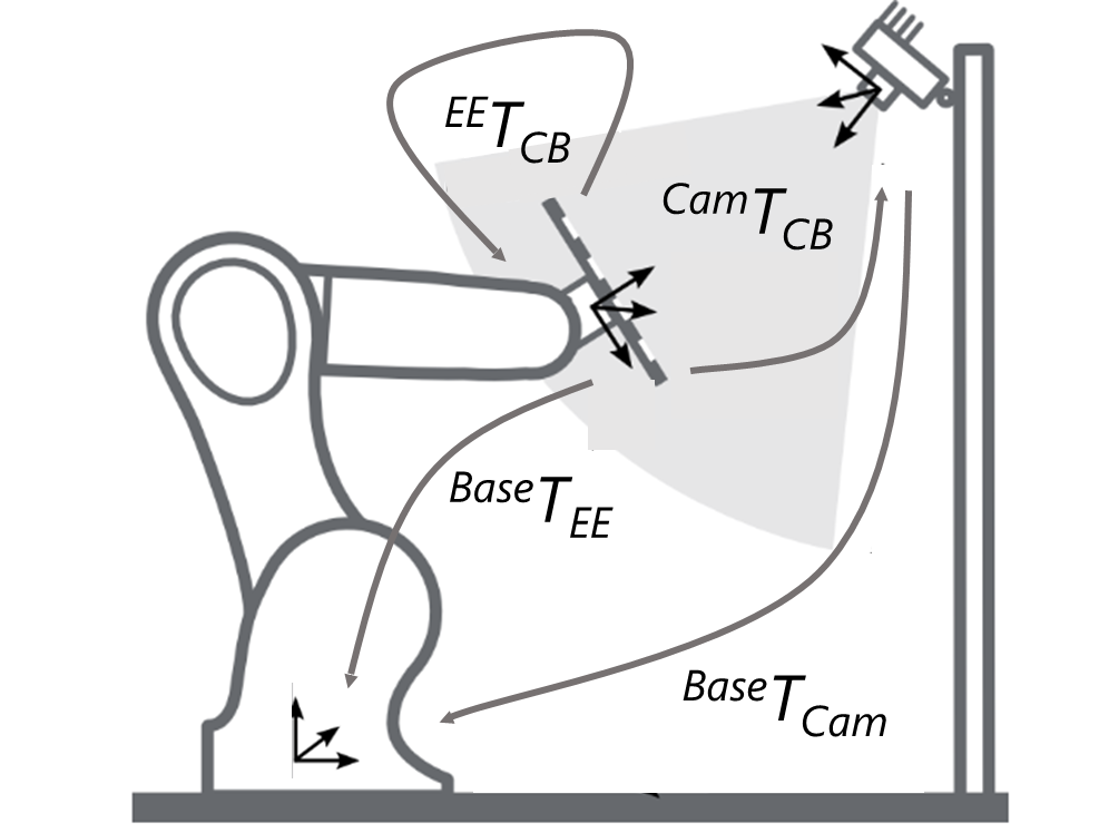
\includegraphics[width=\linewidth]{Handeye}
 	\caption{Hand eye setup}
 	\source{\cite{WinNT} (modified)}
 	\label{Handeyecalibrationsetup}
 \end{figure}


Figure \ref{Handeyecalibrationsetup} depicts the robot and camera set up required for hand-eye calibration. There are four transformations, namely end  to base  ${}^{Base}T_{EE}$, chessboard to end effector  ${}^{EE}T_{CB}$, chessboard to camera  ${}^{Cam}T_{CB}$ and camera to base  ${}^{Base}T_{Cam}$. Defining new variables  ${}^{Base}T_{EE}$ as M,  ${}^{EE}T_{CB}$ as X,  ${}^{Base}T_{Cam}$ as Y and  ${}^{Cam}T_{CB}$ as N we can write the transformation equation as 
\begin{equation}
    MX = YN
    \label{eqn:HandEye}
\end{equation}
% #TODO Why do you name them in one way and then define other names in the next sentence? - to be consistance with the cited paper.

M is obtained through forward kinematics, N is obtained by calculating the pose of the calibration pattern from the camera image. 
As the equation system \ref{eqn:HandEye} is underdetermined, we need several different poses to be able to get a solution. We defined over 60 different poses, always making sure that the chessboard is completely visible in the camera image. The calibration process is automated. The robot drives to each of the defined positions where an image was taken using the RGB camera. The pose of the chessboard in camera coordinates is determined for each position by using the camera extrinsic calibration.


Hand eye calibration aims to solve the two unknowns in (\ref{eqn:HandEye}) i.e the chessboard position with respect to the robot's end effector X and the camera position with respect to the robot's base Y. The equation is transformed to the form Aw = b as presented in the equations (4), (5) and (6) of \cite{ernst2012non}. However, $N_i$’s in the equation (6) of \cite{ernst2012non} is replaced by inverse of $N_i$’s. Non trivial elements of matrices X and Y were computed by solving Aw = b in a least square method.


\subsection{Head Tracking [SP]}

In order to facilitate the tracking of head movement, we need to obtain three-dimensional data of the head and process it further. The Kinect depth camera provides head data for geometric alignment. Iterative Closest Point (ICP) algorithm is widely used to align the three dimensional models when an initial estimate of the relative pose is known.

Inputs for ICP registration are two point clouds and an initial transformation that aligns the source point cloud with the target point cloud approximately. We evaluated two variants of ICP registration named point-to-point ICP and point-to-plane ICP. 
After preliminary trials, we decided to use the point-to-plane method, which is based on an algorithm by Yang Chen $\cite{chen1992object}$ to register our point clouds since it achieves quicker convergence.

In general, ICP iterates over 2 steps:
\begin{enumerate}[leftmargin=*]
    \item Find correspondence set $S=\{p,q\}$ from target point cloud $p$ and source point cloud $q$ which is transformed with current transformation matrix $T$.
    \item Update the transformation $T$ by minimizing the objective function $E(T)$ \eqref{eqn:objective_fn} which is defined over correspondence set $S$.
\end{enumerate}
\begin{equation}
E(T)=\sum_{p,q\subset{S}}{((p-Tq)\cdot n_p)^2}
\label{eqn:objective_fn}
\end{equation}
$n_p$ is the normal of point $p$ \cite{rusinkiewicz2001efficient} in objective function $E(T)$. The point-to-plane approach needs estimation of plane normals. The algorithm finds  adjacent points and calculates the principle axis of adjacent points using covariance analysis. Internally, this algorithm uses jacobian matrices and computes residuals of the point-to-plane ICP objective.

We employ the open source library Open3D \cite{Open3D}, which provides point cloud processing and an implementation of point-to-plane ICP.
 
% \lipsum[1] % Dummy text

\subsection{Implementation [LK]}
We combine the head tracking with matrices from calibrations and inverse kinematics to create a tracking system as shown in fig. \ref{Implementation}.

\begin{figure}[ht]
	\centering
 	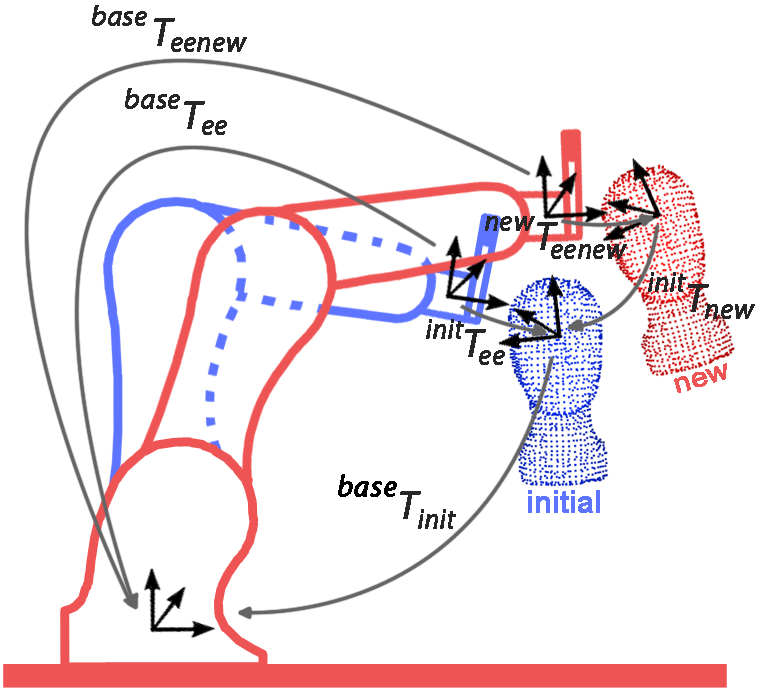
\includegraphics[width=\linewidth]{implementation2}
 	\caption{Transformations used for tracking}
 	\label{Implementation}
 \end{figure}

Raw point cloud data is preprocessed to remove outlier points which are not part of the face geometry by using thresholds and color filters. In figure \ref{Implementation} two head point clouds are shown, where the blue one is the initial one saved at the beginning.

The matrix from the hand eye calibration ${}^{Base}T_{Cam}$ is multiplied and combined with the initial head offset from the camera to calculate a transformation ${}^{Base}T_{Init}$, which is fixed during tracking. Also an inital offset ${}^{Init}T_{EE}$ of the endeffector from the head is calculated using ${}^{Base}T_{Init}$ and forward kinematics. 

When tracking a new pose, Open3D point-to-plane ICP is used to obtain a transformation matrix between the initial head position and the current one called ${}^{Init}T_{New}$. 
\begin{equation}
{}^{Base}T_{EEnew}={}^{Base}T_{Init} {}^{Init}T_{New} {}^{Init}T_{EE}
\label{eqn:implementation}
\end{equation}
These matrices can be multiplied as seen in \eqref{eqn:implementation} to obtain the matrix ${}^{Base}T_{EEnew}$ which is translated into joint angles with the use of inverse kinematics. 

% \lipsum[1] % Dummy text
 % load section from separate file to make everything a bit more clear
%------------------------------------------------
% !TEX root = paper.tex
\section{Evaluation}

We evaluate both the tracking system and the calibration to quantize the tracking error and locate the main sources of inaccuracies.
%\lipsum[1] % Dummy text

\subsection{Evaluation of Tracking [SE]}

As we used a closed form solution for the inverse kinematics, the robot movements itself can be seen as accurate. 
The main source for errors is therefore, apart from imperfect hand-eye calibration, the head tracking. To evaluate the accuracy of the head tracking, we mounted the head on the UR5 and used the touch panel to move it accurately along each axes. 
As the coordinate systems of the UR5 and the camera did not align, we only considered relative movement based on the standing head at the beginning of each measurement. We expected the head tracking result to vary in a small intervall around the actual value while the robot was not moving. For a moving head we expected that the tracking would lag behind but reach the correct final value. 

These assumptions were confirmed in many of the measurements. As expected, lower speeds  delivered in general better results. For some movements we experienced that the tracking system could not catch up with the robot. After the completion of the movement, a static error remained. Figure \ref{fig:z70} displays this behavior. The upper plot shows the actual movement in blue and the predicted movement in orange. The lower plot shows the absolute error, so the differences between both curves. 

\begin{figure}[ht]
    \centering
    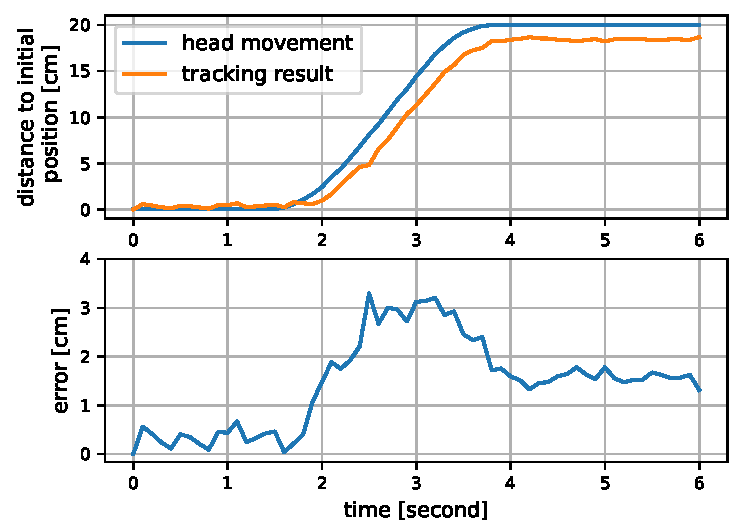
\includegraphics[width=\linewidth]{tracking_eval_z70}
    \caption{Movement along Robot z axes, 70\% speeds}
    \label{fig:z70}
\end{figure}

The best results were achieved for movements in robot $y$ axes. Even at 100\% speed we got surprisingly low errors. A reason for that might be, that nearly all the complete movement in that direction took place towards or away from the camera. Therefore the movement could be well identified by the IR depth sensor. Figure \ref{fig:y100} shows the measurements for that case. 


\begin{figure}[ht]
    \centering
    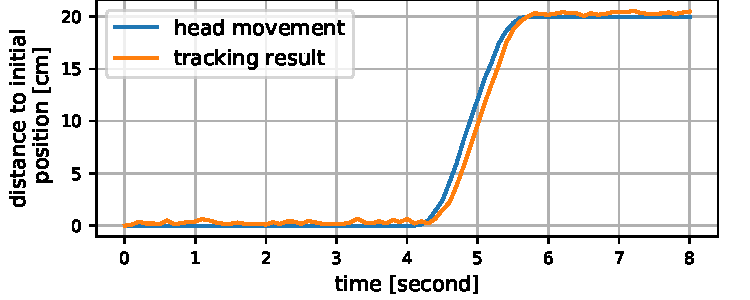
\includegraphics[width=\linewidth]{tracking_eval_y100_single}
    \caption{Movement along Robot y axes, 100\% speeds}
    \label{fig:y100}
\end{figure}

Table \ref{tab:rmse} shows the root-mean-square error (RMSE) for each measurement. A control measurement with a not moving head resulted in a RMSE of 0.069 cm. The extremely high error for axes x at 100\% speed is likely to be caused by some error in the test setup and not part of the normal performance of our system. Due to the limited time with the robot, we were not able to additional testing to confirm or refute this value. 


\begin{table}[hbt]
    \caption{RMSE [cm] of head tracking}
    \centering
    \begin{tabular}{l|cccc}
        \toprule
        & \multicolumn{4}{c}{speed [\%]} \\
        Axes & 30 & 50 & 70 & 100 \\
        \midrule
        x & 1.789 & 0.880 & 1.671 & 4.701 \\
        y & 0.431 & 0.614 & 0.736 & 0.801 \\
        z & 0.453 & 0.482 & 1.744 & 1.863 \\
        \bottomrule
    \end{tabular}
    \label{tab:rmse}
\end{table}

The big differences for the different axes suggest that intelligent placement of the camera is very important. The camera should if possible be placed in line with the biggest expected movement.  

\subsection{Accuracy of Hand-Eye Calibration [PV]}

From equation \eqref{eqn:HandEye} it is easy to see that the transformation from robot base to its own base in a loop (through M,N,X,Y) is identity. This fact is taken as a measure of the quality of the hand eye calibration. The RMS value of the positional error for the 10 poses that are far apart from each were calculated and standard deviation of these 10 RMS values is $\sigma = 0.00329$. There is a scope to improve the handeye calibration accuracy.  

%\lipsum[1] % Dummy text

%\lipsum[1] % Dummy text

%------------------------------------------------
% !TEX root = paper.tex
\section{Conclusion [LK, MH]}

Using our test setup we were able to verify the functionality of an image guided motion compensation system for TMS. 
We achieved a tracking error of below 1 cm for many of the motion tests.
Although we have improved our tracking accuracy a lot during development it is not enough for clinical use by a large margin.
Our current system also performs a lot worse for rotational movement compared to translations, which should be considered for future work.
We would like to compare our system to the error of a handheld coil to see how much improvement can be yielded using a robot.
Further improvements can be made by using a head model as comparison input for the ICP algorithm or using a Neural Network for registration instead of ICP.

% \lipsum[1] % Dummy text

%----------------------------------------------------------------------------------------
%	REFERENCE LIST
%----------------------------------------------------------------------------------------
\phantomsection
\bibliographystyle{unsrt}
\bibliography{sample}

%----------------------------------------------------------------------------------------

\end{document}